\paragraph{Coordinate comparison.}
The script \texttt{check\_coordinate\_obstruction.py} evaluates
Proposition~\ref{prop:coordinate-same-source} at
$m\in\{4,8,16,32,64,128,256,512\}$. It uses exactly the polynomial
$G_m$, the locations $(0,1/2,1)$, and source weights proportional to
$(1,\eta,\eta^2)$, with the explicit finite choice
$\eta=10^{-3}m^{-4}$. With $P_L$ merging the first two points and $P_R$
the last two, the reported quantity
\[
 \mathcal K_m=\frac{D_\varphi(P_L)}{V_h(P_L)}
              \frac{V_h(P_R)}{D_\varphi(P_R)}
\]
is a lower bound on any all-partition comparison factor $C/c$ for that
source. It is not a hierarchy price. The three-state hierarchy price is
exactly one by the analytic argument in the proposition.

\begin{table}[ht]
\centering\small
\begin{tabular}{@{}rrrr@{}}
\toprule
$m$ & Curvature degree $r$ & $\mathcal K_m$ & Normalized $\OPT_2$\\
\midrule
4   & 12   & 4.37840 & $4.35994\times10^{-14}$\\
16  & 60   & 79.7071 & $7.11253\times10^{-21}$\\
64  & 252  & 1669.19 & $7.11649\times10^{-28}$\\
256 & 1020 & 33733.2 & $5.98140\times10^{-35}$\\
512 & 2044 & 149434  & $1.67346\times10^{-38}$\\
\bottomrule
\end{tabular}
\caption{Selected finite coordinate-comparison checks. Every row has
actual all-capacity hierarchy price one. Curvature is divided by
$m^4+m^2$, a global upper bound on $G_m$, so it is at most one.
The comparison ratios are unchanged by this normalization.}
\label{tab:coordinate-check}
\end{table}

Integrals use Gauss--Legendre orders 96 and 192 separately on panels
formed from the trigonometric zeros and dyadic endpoint subdivisions.
The largest observed relative discrepancy between the two orders in
the recorded quantities is $2.89\times10^{-15}$. This checks numerical
stability on the finite set; it is not an interval certificate.
The very small flat costs in Table~\ref{tab:coordinate-check} also show
why comparison ratios should be accompanied by their absolute scales.
An independent check expands the Chebyshev recurrence into polynomial
coefficients at $m=4,16$, evaluates the Bregman moments by polynomial
antiderivatives, and integrates $\sqrt{G_m}$ adaptively with 100-digit
arithmetic. This independent check covers the four basic interval
quantities (two coordinate lengths and two directed divergences); it
does not separately recompute the tiny weighted partition costs.
Its largest relative discrepancy from the panel quadrature
is $2.25\times10^{-15}$; it too is not interval arithmetic.

\begin{figure}[ht]
\centering
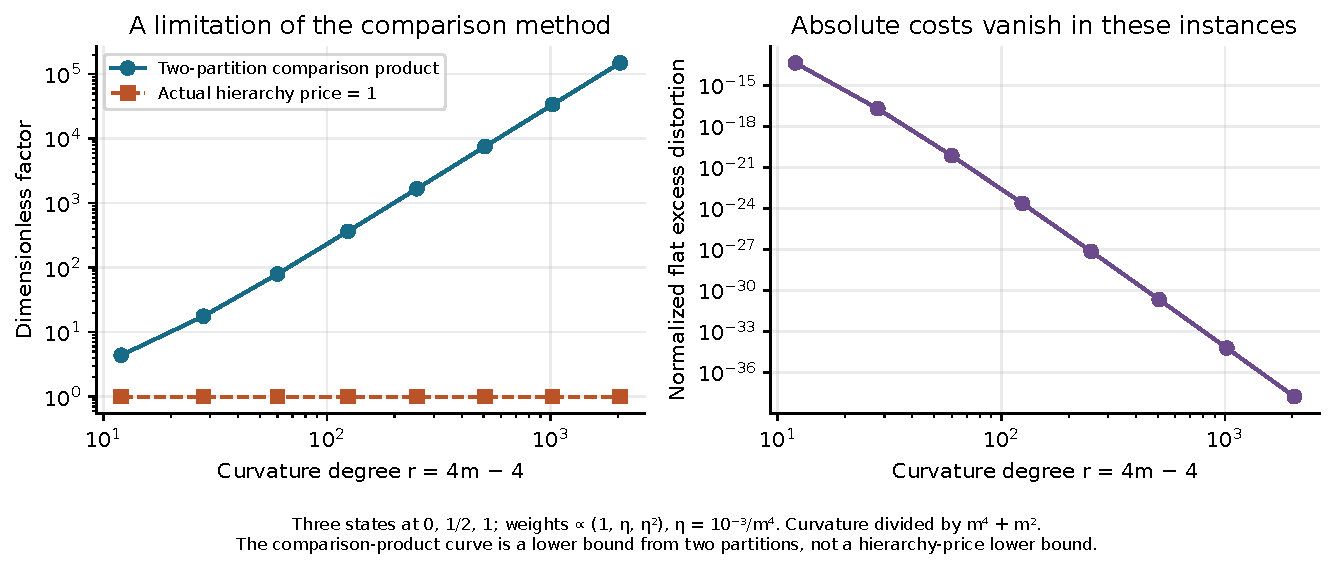
\includegraphics[width=\textwidth]{coordinate_method_obstruction.pdf}
\caption{The same finite examples: the two-partition comparison product
grows while the actual hierarchy price stays one (left), and the
normalized flat distortion becomes very small (right). Lines connect
computed points; no asymptotic fit is used.}
\label{fig:coordinate-check}
\end{figure}
